\documentclass[a4paper,twocolumn]{IEEEtran}
\usepackage{cite}
\usepackage{graphicx}
\usepackage{amsmath}
\usepackage{amssymb}
\usepackage{bm}
\usepackage{amsthm}
\usepackage{cases}
%\usepackage[numbers,sort&compress]{natbib}

\newtheorem{definition}{\textbf{Definition}}
\newtheorem{proposition}{\textbf{Proposition}}
\newtheorem{corollary}{\textbf{Corollary}}
\newtheorem{remark}{\textbf{Remark}}
\newtheorem{lemma}{\textbf{Lemma}}
\newtheorem{theorem}{\textbf{Theorem}}
\newtheorem{example}{\textbf{Example}}

\begin{document}
\title{ECE869 Project: Downlink Interference Analysis in Heterogeneous Cellular Networks using Stochastic Geometry}
\author{\IEEEauthorblockN{Yuan Liang}\\
	\vspace{6pt}
	\IEEEauthorblockA{Department of Electrical \& Computer Engineering, Michigan State University\\ East Lansing, MI 48824, USA.\\Email: liangy11@msu.edu}}
\maketitle

\begin{abstract}
	Stochastic geometry is a mathematic tool that has been used in the analysis of ad hoc networks to model the distribution nodes for more than three decades. Recently, people start to apply stochastic geometry to heterogeneous networks to provide tractable results in network evaluation. In this paper, we briefly introduce the basic concepts in stochastic geometry and the literature on the topic. A toy example is given to illustrate the applicability of stochastic geometry in heterogeneous network. It is shown that stochastic geometry can greatly simplify the analysis. The results also demonstrate the advantage of universal frequency reuse in heterogeneous networks.
\end{abstract}

\section{Introduction}
With the rapid development of smart phones, tablets and wearable devices, the demand for Internet connectivity in wireless cellular networks upsurges dramatically in recent years. The traditional homogeneous network expansion technique, such as cell splitting, is inept at handling such a growth since the deployment of macro base station (MBS) necessitates a huge capital expenditure (CAPEX). Under such circumstance, industries start to resort to other solutions, and the concept of small cells is proposed and has been included in 3G, LTE and WiMax standards\cite{Lin2011}.

The term ``small cell'' refers to the low-power and low-cost radio access points operating in both licensed and unlicensed spectra. Compared to typical mobile macrocells which have ranges of up to several kilometers, the small cells may have ranges from several meters to several hundred meters. And different from the unlicensed small cells, such as Wi-Fi hot spot, small cells, including femtocells, picocells, microcells and metrocells, can provide service in both licensed and unlicensed bands with higher quality of service (QoS).

In order to reduce the CAPEX and operational expenditure (OPEX) of service providers, some small cells, e.g. femtocells, are deployed and managed by users. Small cells will offload a certain percentage of traffic from macro network and thus improve the network capacity. The network constituted by the MBSs overlaid by the small cell base stations (SBSs) is called a heterogeneous network (also referred to as a multi-tier cellular network).

In order to accommodate more users with limited wireless spectrum resources, universal frequency reuse is often employed in heterogeneous networks\cite{Lin2011, Andrews2012JSAC}. That is, the available spectrum will be aggressively reused by all of the network tiers. This strategy reduces the extra cost of network coordination at the expense of increased interference in both intra-tier and cross-tier. From a information theory perspective, the signal to interference and noise ratio (SINR) plays a fundamental role in determining the capacity of channel. Thus the analysis of interference is of special interest in heterogeneous networks.

Conventionally, the distribution of base stations (BSs) in homogeneous networks is assumed to follow a hexagonal grid model. However, such assumption in heterogeneous networks is not suitable because (i) the interference analysis may require massive Monte Carlo simulation\cite{Gilhousen1991} which is intractable and (ii) due to the variation in demand among areas, the distribution of BSs in heterogeneous networks will have random patterns. Thus, new models for heterogeneous cellular networks are needed.

Recently, a new modeling approach basing on stochastic geometry is adopted in heterogeneous networks which can lead to tractable analytical results while keeping the randomness of network geometry. Stochastic geometry is a very powerful mathematical and statistical tool for the modeling, analysis and design of wireless networks with random topologies and has been applied in ad hoc networks for several decades\cite{Haenggi2013Book, Haenggi2009JSAC, Baccelli2009Vol1, Baccelli2009Vol2, Cardieri2010}.

In this paper, we will give a brief introduction of some most basic concepts in stochastic geometry and its application in heterogeneous networks. We will also demonstrate the modeling of heterogeneous networks via a simple downlink interference analysis in a two tier cellular network using stochastic geometry. We wish to illustrate the applicability of stochastic geometry in network modeling and analysis by this paper.

The rest of the paper is organized as follows. Section \ref{Sec:Preli} will present some basic concepts and theorems in stochastic geometry. Section \ref{Sec:Rel} will introduce a few literature on heterogeneous networks using the technique. A simple yet illustrative example of downlink interference analysis in a two-tier cellular network will be discussed in section \ref{Sec:Int} followed by the simulation results in section \ref{Sec:Num}. Finally, section \ref{Sec:Con} will conclude the paper.           
\section{Preliminaries}\label{Sec:Preli}
Consider $d$-dimensional Euclidean space $\mathbb{R}^d$. A spatial \emph{Point Process} (PP) $\Phi$ is a random, finite or countably-infinite collection of points in the space $\mathbb{R}^d$, without accumulation points. $\Phi$ is often expressed in the form of counting measure of PP, which is
\begin{displaymath}
\Phi = \sum_i \varepsilon_{\bm{C}_i}
\end{displaymath} 
where $\bm{C}_i$ is the coordinate of the $i$-th point in PP and $\varepsilon_{\bm{c}}$ is the \emph{Dirac measure} at location $\bm{c}$, i. e., for $A \subset \mathbb{R}^d$, $\varepsilon_{\bm{c}}(A)=1$ if $\bm{c} \in A$ and $\varepsilon_{\bm{c}}(A)=0$ otherwise. So $\Phi(A)$ is the number of points of PP in area $A$. For any function $f$ defined on $\mathbb{R}^d$, there is   
\begin{displaymath}
\sum_i f(\bm{C}_i) = \int_{\mathbb{R}^d}f(\bm{c})\Phi(d\bm{c}).
\end{displaymath}
Following gives the definition of Poisson Point Process (PPP).
\begin{definition}
A Poisson Point Process $\Phi$ of intensity measure $\Lambda$ is defined by
\begin{equation}
\Pr\{\Phi(A_1) = n_1, ..., \Phi(A_k) = n_k\} = \prod_{i=1}^{k} e^{-\Lambda(A_i)}\frac{\Lambda(A_i)^{n_i}}{n_i !}
\end{equation}
for all the possible bounded and mutually disjoint sets $A_i$, $i = 1,2, ..., k$, where intensity measure $\Lambda(A_i)$ is the mean number of points in $A_i$. If $\Lambda(d\bm{c}) = \lambda d\bm{c}$, we call $\Phi$ a homogeneous PPP with intensity $\lambda$.  
\end{definition}

Following is an important property of PPP.
\begin{lemma}
	Given there are $n$ points in the set $W$, these points are independently and identically distributed (i.i.d) in W according to the law $\frac{\Lambda(\cdot)}{\Lambda(W)}$
\end{lemma}
\begin{proof}
	Let $A_1, ..., A_k$ be an arbitrary partition of $W$, where $A_i \cap A_j = \varnothing$ for $j \neq i$ and $\cup_i A_i = W$. For all $n$, $n_1$, ..., $n_k$ with $\sum_i n_i = n$,
	\begin{eqnarray}
	&&\Pr\{\Phi(A_1) = n_1, ..., \Phi(A_k) = n_k | \Phi(W) = n\}\nonumber\\
	&=&\frac{n!}{\Lambda(W)^n}\prod_{i=1}\frac{\Lambda(A_i)^{n_i}}{n_i!}\nonumber
	\end{eqnarray}
\end{proof}

Under many circumstances, the Laplace functional of PP is often needed in analysis.
\begin{definition}
The Laplace functional $\mathcal{L}$ of a PP $\Phi$ is defined as
\begin{displaymath}
\mathcal{L}_{\Phi}(f) = \mathbf{E}\left[ e^{-\int_{\mathbb{R}^d} f(\bm{c}) \Phi(d \bm{c})}\right]
\end{displaymath}
for some non-negative function $f$ on $\mathbb{R}^d$.
\end{definition}
\begin{proposition}\label{Proposition:LaplacePPP}
The Laplace functional of PPP with intensity measure $\Lambda$ is
\begin{equation}
\mathcal{L}_{\Phi}(f) = e^{-\int_{\mathbb{R}^d}(1-e^{-f(\bm{c})})\Lambda(d \bm{c})}
\end{equation}
\end{proposition}
\begin{proof}
See \cite[Proposition 1.2.2]{Baccelli2009Vol1}.
\end{proof}

Some transformations can be applied to a PP.
\begin{definition}[\textbf{Superposition}]
The superposition of PP $\Phi_k$ is defined as the sum $\Phi=\sum_k \Phi_k$. 	
\end{definition}
\begin{proposition}
The superposition of independent PPP with intensities $\Lambda_k$ is a PPP with intensity measure $\sum_k \Lambda_k$ if and only if the latter is locally finite measure.
\end{proposition}	
\begin{proof}
See \cite[Proposition 1.3.3]{Baccelli2009Vol1}.
\end{proof}
\begin{definition}[\textbf{Thinning}]
The thinning of $\Lambda$ with the retention function $p$ is a PP given by
\begin{displaymath}
\Lambda^p = \sum_i \delta_i \varepsilon_{\bm{C}_i} 
\end{displaymath}
where the random variables $\delta_i$ are independent given $\Phi$, and $\Pr\{\delta_i=1\mid \Phi\}=1-\Pr\{\delta_i=0\mid \Phi\}=p(\bm{C}_k)$.
\end{definition}
\begin{proposition}\label{prop:PPPthinning}
The thinning of the PPP of intensity measure $\Lambda$ with retention probability $p$ yields a PPP of intensity measure $\Lambda'$ with $\Lambda'(A)=\int_A p(\bm{c}) \Lambda(d\bm{c})$.
\end{proposition}
\begin{proof}
See \cite[Proposition 1.3.5]{Baccelli2009Vol1}.
\end{proof}
In the analysis of wireless network, it is of special interest to model the distribution of other points in PP given a point at a certain location.
\begin{definition}[\textbf{Palm theory}]
Consider a PP $\Phi$ with a locally finite mean measure. The Palm version of $\Phi$, $\Phi_{\bm{c}}$, is defined given there is a point at $\bm{c}$. And the reduced Palm version $\Phi_{\bm{c}}^!$ is the PP removing point at $\bm{c}$ in $\Phi$.  
\end{definition}
\begin{theorem}[\textbf{Slivnyak-Mecke Theorem}]
For a PPP $\Phi$, its reduced Palm version $\Phi_{\bm{c}}^!$ is equal to its original distribution, i.e., $\Phi_{\bm{c}}^! = \Phi$ and $\Phi_{\bm{c}} = \Phi+\varepsilon_{\bm{c}}$ for all $\bm{c}\in\mathbb{R}^d$.    
\end{theorem}
\begin{proof}
See \cite[Theorem 1.4.5]{Baccelli2009Vol1}.
\end{proof}
In addition, stationarity of a PP is also defined.
\begin{definition}[\textbf{Stationarity}]
A PP $\Phi$ is stationary if its distribution is invariant under translation through any vector $\bm{v}\in\mathbb{R}^d$, i.e. $\Pr\{\bm{v}+\Phi \in \Gamma\}=\Pr\{\Phi \in \Gamma\}$, where $\bm{v}+\Phi=\bm{v}+\sum_i \varepsilon_{\bm{C}_i} = \sum_i \varepsilon_{\bm{v}+\bm{C}_i}$.
\end{definition}
\begin{proposition}
A homogeneous PPP is stationary.
\end{proposition}
\begin{proof}
See \cite[Proposition 1.6.2]{Baccelli2009Vol1}.
\end{proof}

\section{Related Works}\label{Sec:Rel}
Stochastic geometry is a mathematical tool that can provide spatial averages for quantities of interest (e.g., interference, SINR, outage probability, and achievable data rate) over a large number of nodes randomly distributed or over many network realizations\cite{Haenggi2009JSAC}. Among the PPs, PPP is the mostly used one because of its tractability in analysis, and has been applied in ad hoc network to model the distribution of nodes for more than three decades\cite{Kleinrock1978}. However, since the points are distributed independently in PPP, which is not a proper characterization of the BSs in cellular networks, stochastic geometry and PPP are not widely used in cellular networks until recently.     

In \cite{Andrews2011TC}, the authors compared the performance of a PPP and a square grid model to the performance of an actual deployed cellular network and showed that PPP can provide a lower bound on the coverage probability and the mean transmission rate obtained by measurements that are as tight as the upper bound provided by the idealized grid-base model. Such comparison revealed the accuracy of PPP model and shed lights on the modeling and analysis of cellular wireless networks using stochastic geometry.

In \cite{Andrews2011TC}, the BSs and users were modeled as independent homogeneous PPPs and all the BSs used same frequency. Users were assumed to be served by the BSs which could provide the highest received signal strength (RSS). In this way, the coverage regions of the BSs would form a Voronoi tessellation\cite{Okabe1992}. The conclusions of \cite{Andrews2011TC} are: (a) the PPP model provides a relatively tight bound for the performance of actual network (b) simple expressions of coverage probability and mean transmission rate can be derived by using PPP model (c) when the noise is negligible in transmission, the SINR statistics are independent of the intensity of BSs.

In \cite{Dhillon2012JSAC}, the authors extended the idea in \cite{Andrews2011TC} to a K-tier cellular network. In the multi-tier cellular network, all network tiers were modeled as independent homogeneous PPPs and all tiers used the same frequency bands. The BSs in different tiers would have different power and thus the network coverage constituted a weighted Voronoi tessellation. The authors computed the tier association probability and the average tier load. It was shown that the PPP assumption is accurate to within $1-2$ dB of the measured coverage probability in an actual LTE network overlaid by heterogeneous tiers modeled as PPPs.

Frequency or channel reuse is a challenging task in stochastic geometry because it may impair the independence among the distribution of the nodes which will lead to a intractable analytical results. In \cite{Andrews2011TC}, the authors overcame this problem by employing a simple frequency reuse scheme, i.e., each BS would randomly and uniformly pick one of th available frequency sub-bands to use, which is equivalent to the independent thinning of PPP. 

However, this simple frequency reuse scheme reduce interference at the expense of decreased spectral reuse efficiency. Fraction frequency reuse (FFR) is a possible alternative which can reduce interference while keeping a high reuse efficiency\cite{Novlan2011TWC}\cite{Novlan2012TC}. In FFR, the cells are spatially partitioned into inner cell region and edge cell region, and different frequency sub-bands are assigned to different regions. The authors in \cite{Novlan2011TWC}\cite{Novlan2012TC} extend the models in \cite{Andrews2011TC} and \cite{Dhillon2012JSAC} to include FFR in single and multi-tier cellular networks. The authors partitioned the inner and edge users basing on the SINR threshold, and in order to keep the PPP property, they assumed that each BS would randomly and uniformly chooses one of the sub-bands for the edge users.

Contrary to spectrum sharing, i.e. universal frequency reuse, which increases spectral efficiency at the expense of higher cross-tier interference, spectrum partitioning eliminates cross tier interference at the expense of lower spectral efficiency. The tradeoff between spectrum sharing and partitioning is of interest in heterogeneous networks. In\cite{Chandrasekhar2009TC}, the available spectrum was partitioned into two group, one assigned to macro tier and the other assigned to femto tier. The MBSs were modeled as a hexagonal grid-based model while the femto access points (FAPs) were modeled by a homogeneous PPP. A randomized spectrum access control called frequency ALOHA (F-ALOHA) was proposed, in which each FAP accessed each of the available frequencies independently with probability $p$. It was shown that the optimum $p$ is a non-increasing function of FAP intensity. In\cite{Cheung2012JSAC}, the authors studied the spectrum sharing/partitioning tradeoffs, aiming at maximizing the transmission capacity subject to an outage probability constraint in a two-tier cellular network. PPP modeling was used in both tiers and it was shown that joint allocation is optimal for sparse network deployments while disjoint allocation is optimal in dense network deployments. In\cite{Chandr2009TWC}, the authors addressed the uplink case in a two-tier cellular network, in which the MBSs were modeled via hexagonal grid, FAPs were modeled via PPP and users were also modeled via PPP. The authors showed that spectrum sharing with sectored antennas along with time hopping spread spectrum boosts the network capacity of the system by a factor of seven relative to the spectrum partitioning with omni-directional antennas.   
\section{Interference Analysis in a Two-Tier Cellular Network}\label{Sec:Int}
In this section, we demonstrate the applicability of stochastic geometry in heterogeneous cellular networks via a toy example on interference analysis in a two-tier cellular network.
\subsection{Model Description}
Consider a two-tier cellular network consisting of macro tier (tier 1) and femto tier (tier 2). The distribution of MBSs and FAPs are independent PPPs $\Phi_1$ and $\Phi_2$ in $\mathbb{R}^2$ (here we consider the 2-dimensional case) with intensities $\lambda_1$ and $\lambda_2$ respectively. Universal frequency reuse and F-ALOHA are employed, i.e., for each available frequency band or channel, each MBS and FAP will randomly access it with probabilities $p_1$ and $p_2$ respectively. No power control is assumed, so in transmission, the received signal power at a distance $r$ from MBS and from FAP are
\begin{equation}
P_i(r)=\frac{P_i \cdot H}{r^\alpha} 
\end{equation}
for $i=1, 2$ respectively, where $P_i$ are constant that stand for the long term received signal power at unit distance from MBS and from FAP respectively, H is a random variable accounting for the random gain of the channel path, and $\alpha$ is the path-loss exponent. Each user will be served by the MBS or FAP the highest long term received signal power of which is highest at the user, equivalent to the MBS or FAP with the smallest weighted distance, where the weighted distance from MBS/FAP is defined as
\begin{equation}
r_{weighted}=r P_i^{-\frac{1}{\alpha}}
\end{equation}

Rayleigh fading is assumed in the model, where $H$ is exponentially distributed with mean $\mu = 1$. It is also assumed that $\alpha = 4$.
\subsection{Interference Analysis}
Consider a user located at an arbitrary position in the network. Because of the stationarity of PPP, it can be assumed, without loss of generality, that the user is located at the origin.
First, we address the distances of the nearest MBS and FAP to the user, denoted by $R_1$ and $R_2$ respectively. Since the two PPPs are independent, the probabilities that the nearest MBS/FAP is at a distance greater than $r$ are
\begin{displaymath}
\Pr\{ R_i > r \} = \Pr\{ \Phi_i(b(r)) =0\} = e^{-\lambda_i \pi r^2}
\end{displaymath}
for $i=1,2$ respectively, where $b(r)$ denotes a ball centered at the origin of radius $r$. So the probability density functions (PDFs) of $R_1$ and $R_2$ are
\begin{equation}
f_{R_i}(r) = 2\lambda_i \pi r e^{-\lambda_i \pi r^2}
\end{equation}
for $i=1,2$ respectively. The PDF of that the user is served by a MBS at distance $r$ is
\begin{eqnarray}\label{Eq:distance_dist}
&&f_{R_1}(r\mid R_1 P_1^{-\frac{1}{\alpha}} < R_2 P_2^{-\frac{1}{\alpha}}) \Pr\{R_1 P_1^{-\frac{1}{\alpha}} < R_2 P_2^{-\frac{1}{\alpha}}\}\nonumber\\
&=&f_{R_1,R_2}(r, r P_1^{-\frac{1}{\alpha}} P_2^{\frac{1}{\alpha}} < R_2)\nonumber\\
&=&f_{R_1}(r) \Pr\{ R_2 > r P_1^{-\frac{1}{\alpha}} P_2^{\frac{1}{\alpha}} \} \nonumber\\
&=&2\lambda_1 \pi r e^{- \pi r^2 [ \lambda_1 + \lambda_2 (\frac{P_2}{P_1})^\frac{2}{\alpha} ] }
\end{eqnarray}
where
\begin{eqnarray}\label{Eq:Prob_Serv}
\Pr\{\text{A user is served by MBS}\}&=&\Pr\{R_1 P_1^{-\frac{1}{\alpha}} < R_2 P_2^{-\frac{1}{\alpha}}\}\nonumber\\
&=&\frac{\lambda_1 {P_1}^\frac{2}{\alpha}}{\lambda_1 {P_1}^\frac{2}{\alpha} + \lambda_2 {P_2}^\frac{2}{\alpha}}
\end{eqnarray} 
And the results for FAP can be easily derived by switching the indices.

Suppose that the user is served by a MBS at distance $r$. Conditioned on this, $\Phi_1(b(r)) = 0$ and $\Phi_2( b( ( \frac{P_2}{P_1} )^\frac{1}{\alpha} r) ) = 0$. For PPPs, the distribution of disjoint sets are independent, so $\Phi_1$ in $\mathbb{R}^2 \backslash b(r)$ and $\Phi_2$ in $\mathbb{R}^2 \backslash b( ( \frac{P_2}{P_1} )^\frac{1}{\alpha} r)$ are still homogeneous PPPs with intensities $\lambda_1$ and $\lambda_2$ respectively. The downlink $SINR$ at the user is 
\begin{equation}
SINR = \frac{P_1 r^{-\alpha} H}{N_0 + \sum_i\sum_j \Delta(\bm{C}_{i,j}) P_i | \bm{C}_{i,j} |^{-\alpha} H(\bm{C}_{i,j})}
\end{equation}
where $N_0$ is the noise power, $\bm{C}_{i,j}$ is the location of the $j$-th BS/AP in $\mathbb{R}^2 \backslash b(r)$ for MBS ($i=1$) and in $\mathbb{R}^2 \backslash b( ( \frac{P_2}{P_1} )^\frac{1}{\alpha} r)$ for FAP ($i=2$), $\Delta(\bm{C}_{i,j})$ is a indicator of whether the BS/AP of tier $i$ located at $\bm{C}_{i,j}$ is using the same frequency band or channel, and $H(\bm{C}_{i,j})$ is random channel gain of the path from $\bm{C}_{i,j}$ to the origin. In the following analysis, noise is omitted, so the term signal interference ratio (SIR) and SINR will be used interchangeably. And $H(\bm{C})$ are assumed to be independent at different locations.
 
Since F-ALOHA protocol is employed, the MBSs and FAPs transmitting in the same frequency band can be modeled as PPPs $\Phi_1'$ and $\Phi_2'$ with intensities $p_1\lambda_1$ and $p_2\lambda_2$ respectively according to proposition \ref{prop:PPPthinning}. Thus the $SIR$ can be denoted by
\begin{equation}
SIR = \frac{P_1 r^{-\alpha} H}{\sum_i\sum_j P_i | \bm{C}_{i,j}' |^{-\alpha} H(\bm{C}_{i,j}')}=\frac{P_1 r^{-\alpha} H}{\sum_i I_i}
\end{equation}
where $\bm{C}_{i,j}'$ are the locations of points in $\Phi_i'$ and  $I_i$ is the aggregate interference from tier $i$. For any realization $\phi_i'$ of $\Phi_i'$ and $h(\bm{c}_{i,j}')$ of $H(\bm{C}_{i,j}')$, the conditional complementary cumulative distribution function (CCDF) of $SIR$ is
\begin{eqnarray}
&&\Pr\{SIR > \theta \mid r, \phi_i',h(\bm{c}_{i,j}') \}\nonumber\\
&=& \Pr \{ H > \theta r^{\alpha} {\sum_i\sum_j \frac{P_i}{P_1} \mid r, \bm{c}_{i,j}' |^{-\alpha} h(\bm{c}_{i,j}')} \mid \phi_i',h(\bm{c}_{i,j}') \} \nonumber\\
&=& e^{-\theta r^{\alpha} {\sum_i\sum_j \frac{P_i}{P_1} | \bm{c}_{i,j}' |^{-\alpha} h(\bm{c}_{i,j}')}}
\end{eqnarray}
So the CCDF of SIR can be denoted by
\begin{eqnarray}
\Pr\{SIR > \theta \mid r\}&=&\mathbf{E}\{ e^{-\theta r^{\alpha} {\sum_i\sum_j \frac{P_i}{P_1} | \bm{C}_{i,j}' |^{-\alpha} H(\bm{C}_{i,j}')}} \} \nonumber\\
&\stackrel{(a)}{=}&\prod_{i} \mathbf{E} \{ e^{- \frac{\theta}{P_1} r^{\alpha} I_i} \} \nonumber\\
&=&\prod_{i} \mathcal{L}_{I_i} (\frac{\theta}{P_1} r^{\alpha})
\end{eqnarray}
where equation (a) results from the independence among the two PPPs. For the Laplace transform of $I_i$. Similar to the proof of Proposition \ref{Proposition:LaplacePPP}, there is
\begin{eqnarray}\label{Eq:Lap_Intf}
\mathcal{L}_{I_i} (t) &=&\lim_{A \rightarrow \mathbb{R}^2} \sum_k e^{-\Lambda_i' (B)} \frac{(\Lambda_i' (B))^k}{k!}\cdot \nonumber\\
&&(\frac{1}{\Lambda_i' (B)}\int_{B}\int e^{-t P_i |\bm{c}|^{-\alpha} h}f(h) dh \Lambda_i'(d\bm{c}))^k \nonumber\\
&=&\lim_{A \rightarrow \mathbb{R}^2} e^{-\Lambda_i' (B)+\int_{B}\int e^{-t P_i |\bm{c}|^{-\alpha} h}f(h) dh \Lambda_i'(d\bm{c})}\nonumber\\
&=&\lim_{A \rightarrow \mathbb{R}^2}  e^{-\int_{B}[1-\int e^{-t P_i |\bm{c}|^{-\alpha} h}f(h) dh] \Lambda_i'(d\bm{c})}\nonumber\\
&=&\lim_{A \rightarrow \mathbb{R}^2}  e^{-\int_{B}[1-\mathcal{L}_H (t P_i |\bm{c}|^{-\alpha})] \Lambda_i'(d\bm{c})}
\end{eqnarray}
where $\Lambda_i'(\cdot)$ is the intensity function of $\Phi_i'$, $B=A\backslash b( ( \frac{P_i}{P_1} )^\frac{1}{\alpha} r)$, and $\mathcal{L}_H(\cdot)$ is the Laplace function of $H$. Since $\Phi_i'$ are homogeneous PPPs with intensities $p_i\lambda_i$, $H$ is exponentially distributed with mean 1 and $\alpha = 4$, (\ref{Eq:Lap_Intf}) can be calculated as
\begin{eqnarray}\label{Eq:Lap_Intf_closed}
(\ref{Eq:Lap_Intf})&=&e^{-2\pi p_i \lambda_i \int_{r\sqrt[4]{\frac{P_i}{P_1}}}^{\infty}\rho\frac{t P_i}{\rho^4 + t P_i}d\rho}\nonumber\\
&=&e^{-\pi p_i \lambda_i \sqrt{t P_i} [\frac{\pi}{2}-\arctan(\frac{r^2}{\sqrt{tP_1}})]} 
\end{eqnarray}
Combining (\ref{Eq:Lap_Intf}) and (\ref{Eq:Lap_Intf_closed}), we can calculate the probability of $SIR$ as well as the outage probability of the user, which is
\begin{equation}
\Pr\{SIR > \theta \mid r\} = e^{-\pi r^2 \sqrt{\frac{\theta}{P_1}} [\frac{\pi}{2}-\arctan(\frac{1}{\sqrt{\theta}})] \sum_i p_i \lambda_i \sqrt{P_i}} 
\end{equation}

For an arbitrary user, by (\ref{Eq:distance_dist}) the CCDF of SIR can be calculated as
\begin{eqnarray}\label{Eq:CCDF_SIR}
&&\Pr\{SIR > \theta \}\nonumber\\
&=&\sum_i \lambda_i \int 2\pi r e^{- \pi r^2 \sum_j (1+p_j \sqrt{\theta} [\frac{\pi}{2}-\arctan(\frac{1}{\sqrt{\theta}})]) \lambda_j \sqrt{\frac{P_j}{P_i}}} dr \nonumber\\
&=&\frac{\sum_i \lambda_i \sqrt{P_i}}{\sum_j (1+p_j \sqrt{\theta} [\frac{\pi}{2}-\arctan(\frac{1}{\sqrt{\theta}})])\lambda_j \sqrt{P_j}}
\end{eqnarray}
From (\ref{Eq:Prob_Serv}) and (\ref{Eq:CCDF_SIR}), it can be concluded that the statistics of SIR in two tiers are identical.

The CCDF of channel capacity of an arbitrary frequency subband can be expressed as
\begin{displaymath}
\Pr\{\ln(1+SIR)>t\}=\Pr\{SIR>e^t-1\}
\end{displaymath}
and it can be easily verified that
\begin{displaymath}
\lim_{t \rightarrow \infty} t \cdot \Pr\{\ln(1+SIR)>t\} = 0
\end{displaymath} 
So the expectation of channel capacity is
\begin{eqnarray}
\mathbf{E}\{\ln(1+SIR)\}&=&\int_{0}^{\infty}\Pr\{\ln(1+SIR)>t\}dt \nonumber\\
&=&\int_{0}^{\infty} \Pr\{SIR>e^t-1\} dt
\end{eqnarray}
Note that the spatial reuse density of each frequency subband is $\sum_i p_i \lambda_i $, then the spatial average of channel capacity is
\begin{equation}
 \sum_i p_i \lambda_i \int_{0}^{\infty} \Pr\{SIR>e^t-1\} dt
\end{equation}
           
\section{Numerical Results}\label{Sec:Num}
In this section, the numerical values of network performance metrics derived in \ref{Sec:Int} will be simulated.

The network parameters are following: the BS/AP intensities are $\lambda_1 = 10^{-6} /\text{m}^2$ and $\lambda_2 = 10^{-4} /\text{m}^2$, the transmitting power of MBS is $10^4$ times higher than that of FAP. In this case, basing on (\ref{Eq:Prob_Serv}), an arbitrary user will be served by MBS or FAP with equal probability, and the statistics of SIR will be equivalent to that in the single tier case with access probability $\frac{p_1+p_2}{2}$. Users are assume to be uniformly distributed over the whole region, so $p_1$ is set to be equal to $p_2$  .

\begin{figure}[t]
	\centering
	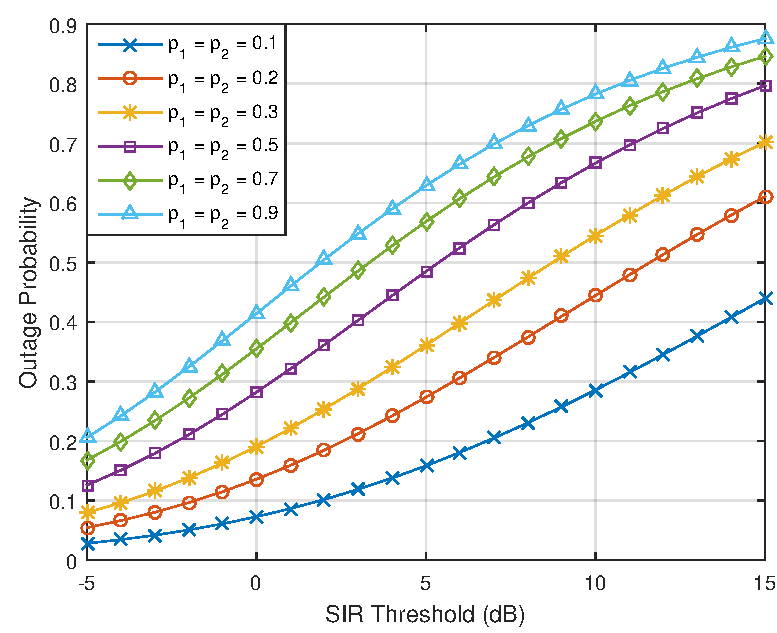
\includegraphics[width = 0.4\textwidth]{figure/Outage_cropped}
	
	\caption{Outage probability of the two-tier network}
	\label{Fig:Outage}
\end{figure}

\begin{figure}[t]
	\centering
	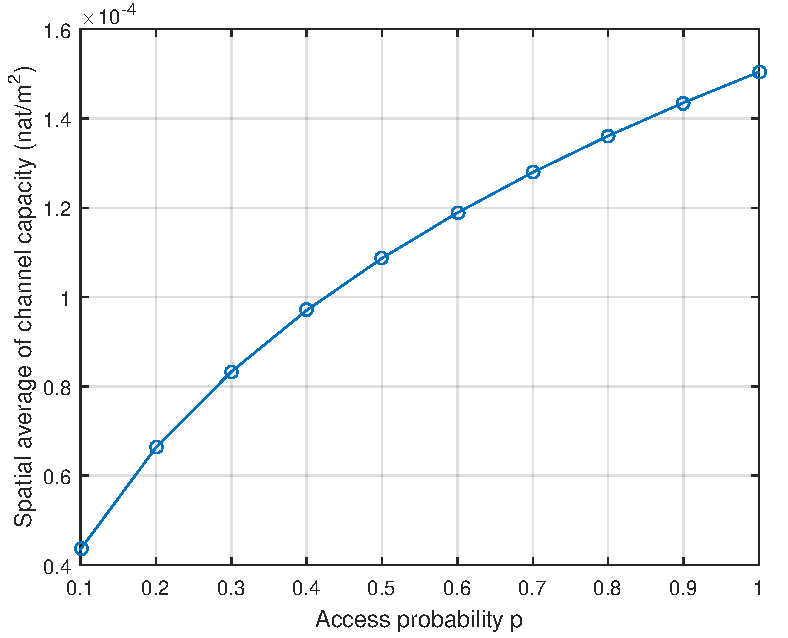
\includegraphics[width = 0.4\textwidth]{figure/Capacity_cropped}
	
	\caption{Spatial average of channel capacity per frequency band}
	\label{Fig:Capacity}
\end{figure}

The outage probability of a channel is defined as the probability that the SIR of the channel is below a certain threshold, which is equivalent to the CDF of the SIR. Fig. \ref{Fig:Outage} gives the numerical values of outage probability for different SIR thresholds and different access probabilities $p_1$, $p_2$. The figure shows that even with a low access probability, the outage probability is still relatively high for high SIR threshold. However, in this toy example, no sophisticated frequency reuse scheme is employed (e.g., FFR and cognitive radio), which could be instrumental in reducing the interference.

Fig. \ref{Fig:Capacity} gives the spatial average of channel capacity in an arbitrary frequency subband. It shows a very interesting result: from a information theory perspective, decreasing the access probability can reduce the interference, though, the channel capacity is also reduced. That is, more opportunities for transmission may outweigh a lower interference for the purpose of pursuing a better overall performance. However, this is only a conclusion in theoretical settings where the ideal channel coding of infinite length is applied, which is not possible in practice. The non-zero channel capacity may not be able to guarantee a valid communication between BS/AP and user when the SIR is too low.    
\section{Conclusion}\label{Sec:Con}
The proliferation of wireless devices necessitates the deployment of a large number of small BSs in wireless cellular network. To model the distribution of these BSs and evaluate the performance metrics of heterogeneous cellular network, stochastic geometry is introduced. In this paper, we introduced some basic concepts in stochastic geometry and some related literature on the topic. A toy example of a two-tier heterogeneous network was given to illustrate the applicability of stochastic geometry. It was shown that with the help of stochastic geometry, closed form expression of the statistics of downlink SIR can be achieved in Rayleigh fading channel with path-loss exponent of $4$, which could greatly simplify the analysis. An interesting result here was that in order to pursue a higher spatial average of channel capacity, each BS/AP of each tier should aggressively access all the available spectra. This substantiates the benefits of universal frequency reuse strategy in heterogeneous networks. However, better schemes in frequency reuse should still be considered to avoid interference for the purpose of providing better QoS to users.      

\bibliographystyle{IEEEtran}
\bibliography{ref}  
\end{document}